% Chapter Template

\chapter{Asymptotic and perturbative methods} % Main chapter title

\label{Chapter2} % Change X to a consecutive number; for referencing this chapter elsewhere, use \ref{ChapterX}

%----------------------------------------------------------------------------------------
%	SECTION 1
%----------------------------------------------------------------------------------------
%In this section, we present various techniques of asymptotics, explain the water wave problem in greater detail, and comment on why we can rely on asymptotics. This chapter assumes familiarity with a basic theory of ordinary and partial differential equations.

In this chapter, we introduce perturbation theory and the most relevant technique for this project, multiple scale analysis. The focus is on the illustration of ideas through examples, rather than rigorous justification and proofs. Examples are adapted from Chapters 7 and 11 of \cite{BO}.

Perturbation theory is a collection of techniques used for obtaining approximate solutions to problems typically involving some small parameter $\epsilon$. The main idea is to represent the unknown variable $f$ as a \textit{perturbation series}, which is a formal power series $f = f_0 + \epsilon f_1 + \epsilon^2 f_2 + \ldots.$ Substituting this expression into the original problem decomposes what is a difficult problem into many simpler ones. Solving for the first $n$ terms in the series yields an approximate solution $f \approx f_0 + \epsilon f_1 + \ldots + \epsilon^n f_n.$ Note that with this approach, perturbation theory is most useful when the first few terms reveal the important features of the solution, and the remaining terms give successively small corrections. Perturbative techniques are applied in numerous settings, including finding roots of polynomials and solving initial value problems for differential equations.

Since we deal with differential equations, in this project we illustrate the perturbation method with an ordinary differential equation (ODE).

\eg{Consider the following boundary value problem (BVP):
\begin{equation}\label{BVP}
y'' + y = \frac{\cos x}{1 + y}, \qquad y(0) = y(\pi/2) = 1. 
\end{equation} 
We introduce a small parameter $\epsilon>0$ into the problem
\[ y'' + y = \frac{\cos x}{1 +  \epsilon y} = \cos x (1 - \epsilon y+ \mathcal{O}(\epsilon^2)),\]
where we use geometric series and introduce asymptotic notation in the last equality (see the Table of Notation for a definition of $\mathcal{O}(\cdot)$). Expanding $y = y_0 + \epsilon y_1 + \mathcal{O}(\epsilon^2)$ and substituting into the above equation gives
\[ (y_0 + \epsilon y_1)'' + y_0 + \epsilon y_1 = \cos x(1 - \epsilon y_0)+ \mathcal{O}(\epsilon^2).\]
By ordering the above in powers of $\epsilon,$ we simplify the original problem into the following two problems:
\begin{align}
\mathcal{O}(\epsilon^0): \qquad &y_0'' + y_0 = \cos x, &y_0(0) = y_0(\pi/2) = 1, \label{S2:s1}\\
\mathcal{O}(\epsilon^1): \qquad &y_1'' + y_1 = - y_0 \cos x, &y_1(0) = y_1(\pi/2) = 0.\label{S2:s2}
\end{align}
Solving \eqref{S2:s1} and \eqref{S2:s2} recursively yields $y_0$ and $y_1:$
\begin{align*}
y_0(x) &=\frac{4\cos x - (\pi - 2 (x + 2)) \sin x}{4}, \\
 y_1(x) &= \frac{2 (-9 + 5 \cos 2x + 14 \sin x) + \cos x (8 - 3 (-4 + \pi - 2 x) \sin x)}{36}.
\end{align*}
An approximate solution becomes $y \approx y_0 + \epsilon y_1 \to y_0 + y_1,$ as $\epsilon \to 1.$ This yields an approximate solution of BVP \eqref{BVP}. Note that as $\epsilon \to 1,$ the geometric series argument is no longer justified; yet, we find an approximate solution whose graph resembles the shape of the exact solution. To improve accuracy, we can proceed to the next order. See Figure \ref{fig:BVP}}\label{S2:ex1}.

\begin{figure}[h]
\captionsetup{width=\textwidth}
\centering
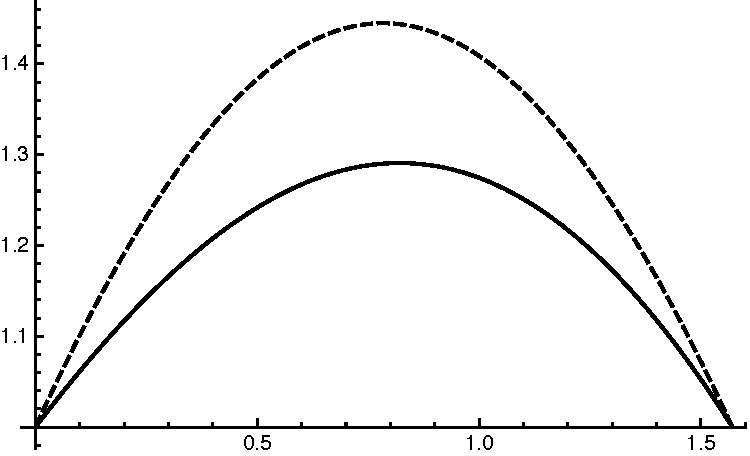
\includegraphics[width=0.65\linewidth]{figures/oneeps.pdf}
\caption[Solutions of nonlinear BVP]{The exact solution $y(t)$ (solid line) of the BVP \eqref{BVP} vs. an approximate solution $y_0 + y_1$ (dashed line), where $y_0$ solves \eqref{S2:s1} and $y_1$ solves \eqref{S2:s2}.}
\label{fig:BVP}
\end{figure}

Although the idea is simple, problems may contain subtleties that require careful analysis before applying the method, as illustrated below. 
\eg{
Consider the following initial value problem (IVP) for the weakly nonlinear Duffing oscillator
\begin{equation}\label{Duffing}
 y'' + y + \epsilon y^3 = 0, \qquad y(0)=1 \qquad y'(0)=0.
\end{equation}
Application of the regular perturbation series yields
\begin{equation}\label{S2:sol}
y(t) \approx y_0 + \epsilon y_1 = \cos t + \epsilon\left(\frac{1}{32} \cos 3t -\frac{1}{32} \cos t + \frac{3}{8} t \sin t\right ),
\end{equation}
which converges as $\epsilon \to 0$ for fixed $t.$ Note that the convergence is only pointwise, not uniform. Indeed, for values $t \sim 1/\epsilon$ or larger, the presence of the \textit{secular}  term $t \sin t$ implies that $y_1$ is unbounded in $t.$ However, solutions of the Duffing oscillator are known to be bounded, so $y_1$ should be bounded. In particular, this suggests that expanding $y$ as a perturbation series is not sufficient, and the secularity is an outcome of this misfortune.}\label{S2:ex2}

\section{Multiple scale analysis}
When ordinary perturbative methods fail to give a uniformly accurate approximation, the method of \textit{multiple scales} is useful. The idea is to introduce a new variable $\tau = \epsilon t.$ Physically, $\tau$ represents a longer scale than $t$, since $\tau$ is not negligible when $t \sim 1/\epsilon$ or larger. Even though $y(t)$ is a function of $t$ alone, through introduction of $\tau,$ $y(t)$ becomes a function of $t$ and $\tau,$ i.e $y(t, \tau).$ As such, the multiple scales seeks solutions as functions of both $t$ and $\tau,$ treating these variables independently. Although an artifice, such treatment in two variables eliminates secularities.

We illustrate the method on the Duffing oscillator in Example \ref{S2:ex2}. Formally, we write $y(t) = Y_0(t, \tau) + \epsilon Y_1(t, \tau) + \mathcal{O}(\epsilon^2).$ 
Using chain rule, we substitute this expansion into \eqref{Duffing} and collect powers of $\epsilon$ to obtain
\begin{align}
\mathcal{O}(\epsilon^0): ~ &\frac{\partial^2 Y_0}{\partial t^2} + Y_0 = 0, \quad &Y_0(0,0) = 1 \quad &\frac{\partial Y_0}{\partial t}(0,0) = 0, \label{S1} \\
\mathcal{O}(\epsilon^1): ~ &\frac{\partial^2 Y_1}{\partial t^2} + Y_1 = - Y_0^3 - 2 \frac{\partial^2 Y_0}{\partial \tau \partial t} \quad &Y_1(0,0) = 1 \quad &\frac{\partial Y_1}{\partial t}(0,0) = -\frac{\partial Y_0}{\partial \tau}(0,0). \label{S2}
\end{align}
The general solution of \eqref{S1} is $Y_0(t, \tau) = B(\tau) e^{it} + B^*(\tau) e^{-it},$ where $B(\tau)$ is a complex function of $\tau$. We can determine $B(\tau)$ by requiring that secular terms do not appear in $Y_1(t, \tau).$ Substituting $Y_0$ into \eqref{S2} gives
\begin{equation}\label{S4}
\begin{aligned}
\frac{\partial^2 Y_1}{\partial t^2} + Y_1 =  \left(-3 B^2 B^* - 2i \frac{\D B}{\D \tau}\right) e^{it} &+ \left(-3 B (B^*)^2 + 2i \frac{\D B^*}{\D \tau}\right) e^{-it}\\
&- B^3 e^{3it}  - (B^*)^3 e^{-3it}.
\end{aligned}
\end{equation}
Notice that $e^{it}$ and $e^{-it}$ appear in the solution of \eqref{S1}, which is also the homogeneous solution of \eqref{S2}. Therefore, unless the coefficients of $e^{it}$ and $e^{-it}$ vanish, $Y_1$ grows in $t.$  To preclude secularity, we must have
\[
-3 B^2 B^* - 2i \frac{\D B}{\D \tau} = 0, \qquad \text{and} \qquad -3 B (B^*)^2 + 2i \frac{\D B^*}{\D \tau} = 0.
\]
The two equations are complex conjugates of each other, so $B(\tau)$ is not overdetermined. Solving for $B(\tau)$ along with the given initial conditions yields $B(\tau) = \dfrac{1}{2} e^{i3\tau/8},$ so that we obtain $Y_0(t, \tau) = \cos \left(t + \dfrac{3}{8}\tau\right).$ Finally, using that $\tau = \epsilon t$ gives an approximate solution 
\begin{equation}\label{S2:sol2}
y(t) = \cos \left[ t\left(1 + \epsilon\frac{3}{8}\right)\right] + \mathcal{O}(\epsilon), \qquad \epsilon \to 0, \quad \epsilon t = \mathcal{O}(1).
\end{equation}
To conclude, while \eqref{S2:sol} approximates $y$ well for $0\leq t \ll \mathcal{O}(1/\epsilon),$ \eqref{S2:sol2} approximates $y$ over a much larger range (see Figure \ref{fig:MSfig}). 

\begin{figure}[h]
\captionsetup{width=\textwidth}
  \begin{subfigure}[t]{\textwidth}
    \centering
    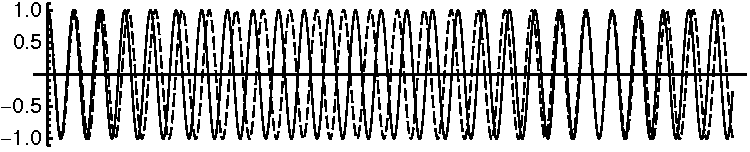
\includegraphics[width=\linewidth]{figures/ExactvsApprox2.pdf}
    \caption{Exact $y(t)$ (solid line) vs. $y(t)=\cos t$ (dashed line)}
    \label{fig:PlotA}
  \end{subfigure}
  \begin{subfigure}[t]{\textwidth}
    \centering
    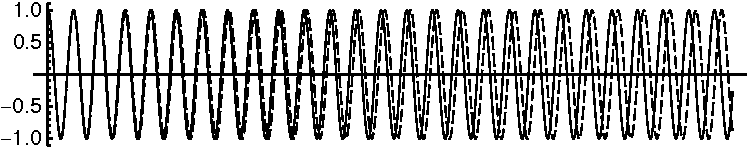
\includegraphics[width=\linewidth]{figures/ExactvsMscales2.pdf}
    \caption{Exact $y(t)$ (solid line) vs. $y(t) = \cos \left[ t(1 + \epsilon\frac{3}{8})\right]$ (dashed line)}
    \label{fig:PlotB}
  \end{subfigure}
  \caption[Solutions of Duffing oscillator IVP]{Superposed solutions of the Duffing oscillator IVP when $\epsilon = 0.1,$ for $t \in [0,160].$ Note that $\cos t$ is not valid for large values of $t;$ at $t = 160, \cos t$ is one cycle out of phase with the exact solution $y(t)$ (Plot \ref{fig:PlotA}). However, multiple scales solution approximates $y(t)$ closely, even for large values of $t$ (Plot \ref{fig:PlotB}).}
  \label{fig:MSfig}
\end{figure}

The choice of scales $\tau = \epsilon t$ tends to be example-specific. In general, one may choose $\tau = f(t; \epsilon),$ where $f$ is some function. For example, for an IVP $\{ y'' + y - \epsilon t y= 0, ~ y(0) = 1, ~ y'(0) = 0 \},$ one uses $\tau = \sqrt{\epsilon} t,$ and for $y''+ \omega^2(\epsilon t) y= 0,$ one uses $\tau = \int^t \omega (\epsilon s) \D s.$ For details, see Chapter 11 of \cite{BO}.

\rmk{It is important to understand the need for multiple scales. For the Duffing oscillator IVP, we could solve the problem numerically, or approximate the solution via multiple scales. A question arises: why use multiple scales when differential equations can be solved numerically? 

Many real-world phenomena are expressed in terms of PDEs, which can be difficult to solve numerically. Due to many differences in the physical phenomena and mathematical challenges, there is no unified analytic and numerical treatment. In addition, developing numerical schemes can be tricky, since issues such as stability, error, and the physical conditions need to be carefully addressed. Furthermore, numerically solving PDEs can be time-consuming and require significant computational power, especially if high precision is required. The latter is particularly important for real-time prediction. This is another reason to prefer multiple scales. When appropriately applied, multiple scales and perturbation methods turn the original, difficult problem into a sequence of simpler problems. These problems are easier to solve either analytically or numerically, and provide further insight into the mathematics and physics of the problem.}
